\chapter{Отношения и функции} 
\label{ch:rel:rel}
%rel: prefix
Отношения и функции являются важнейшими понятиями математики и активно используются для решения практических задач. Для углубленного изучения рекомендуются \cite{bib:sudoplatov:discrmath, bib:haggard:discrmathprogrammer}.


\section{Отношения}

При решении практических задач порой необходимо выбирать элементы, связанные некоторым соотношением.


\emph{$n$-местным отношением} или \emph{$n$-местным предикатом} $P$ на множествах $A_1, A_2, \ldots, A_n$ называется любое подмножество прямого произведения $A_1\times A_2\times \cdots\times A_n$.

Говорят, что элементы $x_1,x_2,\ldots,x_n$ (где $x_1\in A_1,x_2\in A_2,\ldots,x_n\in A_n$) связаны соотношением $P$ (обозначается $P(x_1,x_2,\ldots,x_n)$) тогда и только тогда, когда $(x_1,x_2,\ldots,x_n)\in P$.

\begin{itemize}
	\item При $n=1$ отношение называется \emph{унарным} или \emph{свойством}. 
	\item При $n=2$ отношение $P$ называется \emph{бинарным}. Если $P\subseteq A\times B$ и $(x,y)\in P$, то пишут также $x\,P\,y$. Примером бинарного отношения может являться отношение $\subseteq$.
	\item Отношение $P\subseteq A^n$ называют \emph{$n$-местным предикатом (отношением) на множестве $A$}. \emph{Двуместным (бинарным) отношением на множестве $\mathbb{R}$} является отношение $\leq$.
\end{itemize}


\section{Бинарные отношения}

Бинарные отношения нашли множество практических применений. Существует несколько способов задать бинарное отношение $P\subseteq A\times B$:
\begin{itemize}
    \item множеством упорядоченных пар из $A\times B$;
    \item точками в декартовой системе координат (где на осях будут отложены элементы $A$ и $B$);
    \item ориентированным графом, в котором вершинам будут соответствовать элементы $A\cup B$, а дугам элементы $(a,b)\in P$;
    \item матрицей смежности, строкам которой соответствуют элементы $A$, столбцам --- элементы $B$, а наличию (отсутствию) пары $(a,b)\in A\times B$ в отношении $P$ соответствует 1 (отсутствию --- 0) на пересечении соответствующих строки и столбца;
    \item перечислением множества смежных элементов: \[\{(a,C)|a\in A,C=\{b|(a,b)\in P\}\}.\]
\end{itemize}

\begin{exampl} Задача.
    На множестве 
        \[M=\{m_1,m_2,m_3,m_4,m_5,m_6\}\] 
    задано бинарное отношение $P\subseteq M\times M$:
    \begin{equation}
        \label{eq:binary}
        \begin{split}
            P=\{
                (m_1,m_2),
                (m_1,m_4),
                (m_2,m_3),
                (m_2,m_4),\\
                (m_2,m_6),
                (m_3,m_1),
                (m_3,m_4),
                (m_4,m_5),\\
                (m_4,m_6),
                (m_5,m_6),
                (m_6,m_1),
                (m_6,m_3)
            \}.
        \end{split}
    \end{equation}
    
    Задайте отношение различными способами.
\end{exampl}

\begin{proof}[Решение]
    Бинарное отношение \eqref{eq:binary} уже задано множеством пар из $M^2$. Представление в декартовой системе координат и ориентированным графом приведены на рисунках \ref{fig:binaryR} и \ref{fig:binaryRGraph} соответственно.
    
    \begin{figure}
        \centering
        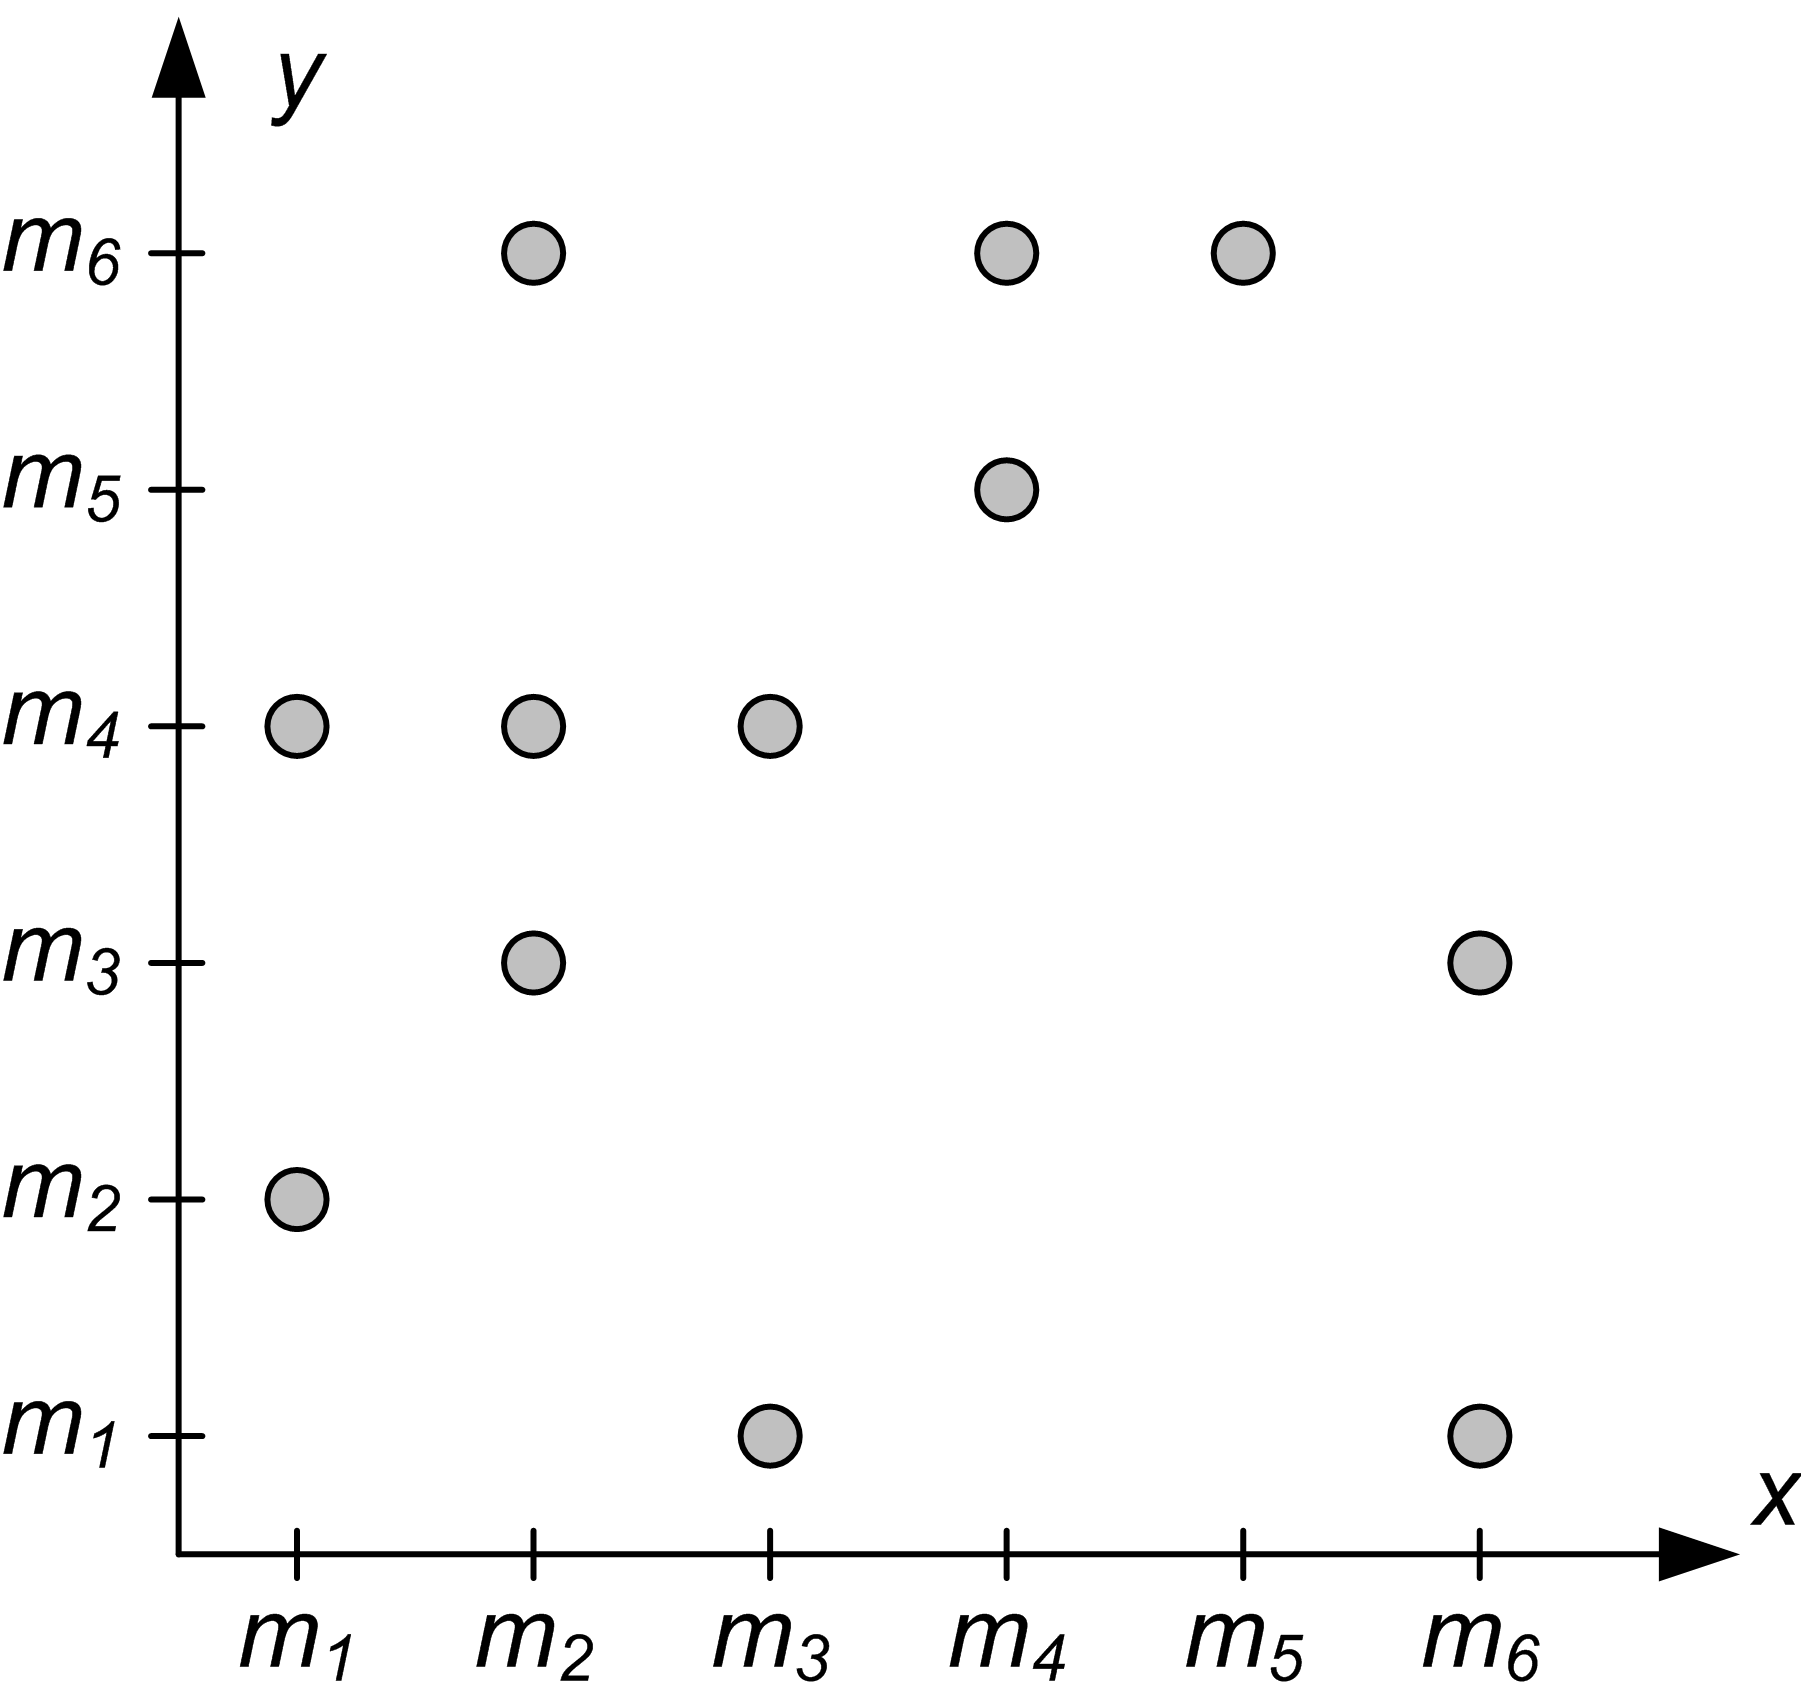
\includegraphics{fig/binaryR}
        \caption{Бинарное отношение в декартовой системе координат}
        \label{fig:binaryR}
    \end{figure} 

    \begin{figure}
        \[
            \xymatrix{
                *{}
                    &m_2 \ar@{->}[r]\ar@{->}[drr]\ar@{->}[dd]
                        &m_3 \ar@{->}[dll]\ar@{->}[dr]
                            &*{}
                                \\
                m_1 \ar@{->}[ur]\ar@{->}[rrr]
                    &*{}
                        &*{}
                            &m_4 \ar@{->}[dl]\ar@{->}[dll]
                                \\
                *{}
                    &m_6 \ar@{->}[ul]\ar@{->}[uur]
                        &m_5 \ar@{->}[l]
                            &*{}
            }
        \]
        \caption{Бинарное отношение задано орграфом}
        \label{fig:binaryRGraph}
    \end{figure} 

    Любое бинарное отношение $P=A\times B$ можно задать матрицей смежности $[P]$, по строкам которой расположены элементы множества $A$, по столбцам --- элементы $B$, а на пересечении строки $a$ и столбцa $b$ стоит 1, если $(a,b)\in P$ и 0 в противном случае. 

    Бинарное отношение \eqref{eq:binary} можно задать следующей \emph{матрицей смежности}\footnote{Договорившись о порядке следования строк и столбцов, шапку матрицы опускают}:

    \[
    [P]=
    \begin{array}{c|cccccc}
           &m_1&m_2&m_3&m_4&m_5&m_6\\ \hline
        m_1&0&1&0&1&0&0\\
        m_2&0&0&1&1&0&1\\
        m_3&1&0&0&1&0&0\\
        m_4&0&0&0&0&1&1\\
        m_5&0&0&0&0&0&1\\
        m_6&1&0&1&0&0&0
    \end{array}=
    \begin{pmatrix}
        0&1&0&1&0&0\\
        0&0&1&1&0&1\\
        1&0&0&1&0&0\\
        0&0&0&0&1&1\\
        0&0&0&0&0&1\\
        1&0&1&0&0&0
    \end{pmatrix}.
    \]

    Любое бинарное отношение $P\subseteq M^2$ можно задать также перечислением множества смежных элементов для каждого $x\in M$. Множество смежных с $x$ элементов определяется так: $\{y|(x,y)\in P\}$. 
    \[
        \begin{array}{c|l}
            \hline\hline
            x\in M&\{y|(x,y)\in P\}\\ \hline\hline
            m_1&\{m_2,m_4\}\\
            m_2&\{m_3,m_4,m_6\}\\
            m_3&\{m_1,m_4\}\\
            m_4&\{m_5,m_6\}\\
            m_5&\{m_6\}\\
            m_6&\{m_1,m_3\}\\ \hline
        \end{array}
    \]
    Бинарное отношение \eqref{eq:binary} будет задано перечислением множеств смежных вершин так:
    \[  
        \begin{split}
            \{
                (m_1,\{m_2,m_4\}), (m_2,\{m_3,m_4,m_6\}), (m_3,\{m_1,m_4\}),\\
                (m_4,\{m_5,m_6\}), (m_5,\{m_6\}),       (m_6,\{m_1,m_3\})\}.
        \end{split}
    \]
\end{proof}

Важными частными случаями \emph{бинарного} отношения на множестве $A$ являются:
\begin{itemize}
    \item \emph{тождественное} отношение (или \emph{диагональ}): $I_A=\{(a,a)|a\in A\}$;
    \item \emph{универсальное} (или \emph{полное}) отношение: $U_A=A^2$.
\end{itemize}

Для бинарного отношения $P$.
\begin{itemize}
    \item \emph{Областью определения} называется множество $\delta_P=\{a|(a,b)\in P\}$.
    \item \emph{Областью значений} называется множество $\rho_P=\{b|(a,b)\in P\}$.
\end{itemize}

\emph{Обратным} к $P$ отношением называется отношение
\[P^{-1}=\{(b,a)|(a,b)\in P\}.\]

\emph{Дополнением} отношения $P\subseteq A\times B$ называется отношение
\[\overline{P}=\{(a,b)|(a,b)\in A\times B\land (a,b)\not\in P\}.\]


\subsection{Композиция и возведение в степень}

Вводится понятие \emph{композиции} (\emph{произведения}) отношений $P_1\subseteq A\times B$ и $P_2\subseteq B\times C$:
\begin{equation}
    \label{eq:binPComposition}
    \begin{split}
        P_1\cdot P_2 = P_1P_2 = \\
        = \{(a,c)|a\in A\land c\in C\land (\exists b\in B (a,b)\in P_1\land (b,c)\in P_2)\}
    \end{split}
\end{equation}

\begin{exampl} Задача. 
    \label{exampl:binPComposition}
    Дано три множества $A=\{g,h\}$, $B=\{1,2,3\}$, $C=\{s,t\}$. Заданы отношения $P\subseteq A\times B$, $Q=B\times C$: 
    \[P=\{(g,1),(g,2),(g,3),(h,2)\},Q=\{(1,t),(2,s),(3,s)\}.\]
\end{exampl}

\begin{proof}[Решение]
    Построим орграф, соответствующий композиции $PQ$. Оба отношения можно задать на одном орграфе:
    \[
    \xymatrix{
        g  \ar@{->}[rr] \ar@{->}[drr] \ar@{->}[ddrr]
            &*{}
                &1 \ar@{->}[ddrr]
                    &*{}
                        &s 
                            \\
        *{}
            &*{}
                &2 \ar@{->}[urr]
                    &*{}
                        &*{}
                            \\
        h \ar@{->}[urr]
            &*{}
                &3 \ar@{->}[uurr]
                    &*{}
                        &t
                            \\
        *{}
            &*{P}
                &*{}
                    &*{Q}
                        &*{}
    }
    \]

    Выполняя композицию:
    \[
        \begin{array}{cc}
        {
            \raisebox{-0.5\height}{
            \(
                \begin{array}{l}
                    g\,P\,1\land 1\,Q\,t\Rightarrow (g,t)\in PQ\\
                    g\,P\,2\land 2\,Q\,s\Rightarrow (g,s)\in PQ\\
                    g\,P\,3\land 3\,Q\,s\Rightarrow (g,s)\in PQ\\
                    h\,P\,2\land 2\,Q\,s\Rightarrow (h,s)\in PQ\\
                    \\
                    PQ=\{(g,t),(g,s),(h,s)\}
                \end{array}
            \)
            }
        }
        &
        {\xymatrix{
                g  \ar@{->}[rr] \ar@{->}[drr]
                    &*{}
                        &s
                            \\
                h \ar@{->}[urr]
                    &*{}
                        &t 
                            \\
                *{}
                    &*{PQ}
                        &*{}
        }}
        \end{array}
    \]
    
    Получим ответ $PQ=\{(g,t),(g,s),(h,s)\}$.
\end{proof}

Для бинарного отношения $P$ на $A$ вводится понятие возведения в степень:
\[
    P^n=
    \begin{cases}
        P^{0}=I_A,\,n=0;\\
        P^{n}=P^{n-1}\cdot P,\,n>0.
    \end{cases}
\]
т.е.
\[
    P^n=\underbrace{P\cdot P\cdot\cdots P}_n.
\]


\subsection{Операции на матрицах смежности}

Пусть $A=\{a_1,\ldots,a_m\}$, $B=\{b_1,\ldots,b_n\}$, $C=\{c_1,\ldots,c_k\}$ и бинарные отношения $P\subseteq A\times B$, $Q=B\times C$ заданы матрицами смежности $[P]_{m\times n}$ и $[Q]_{n\times k}$.

Матрица их композиции $[PQ]_{m\times k}$ называется \emph{логическим} или \emph{булевым} произведением матриц исходных отношений $[P]_{m\times n}\cdot [Q]_{n\times k}$.

Каждый элемент матрицы композиции получается по формуле
\[
    [PQ]_{i,j}=\bigvee_{l=1}^{n} [P]_{i,l}\land [Q]_{l,j},
    1\leq i\leq m, 1\leq j\leq k,
\]
где $\bigvee$ обозначает групповое логическое <<ИЛИ>>.

\begin{exampl}
    \label{exampl:binPcompositionMatrix}
    Для отношений из примера \ref{exampl:binPComposition} матрицы смежности:
    \[
        [P]_{2\times 3}=
        \begin{array}{c|ccc}
              & 1 & 2 & 3 \\ \hline
            g & 1 & 1 & 1 \\
            h & 0 & 1 & 0
        \end{array}=
        \begin{pmatrix}
            1&1&1\\
            0&1&0
        \end{pmatrix},\,
        [Q]_{3\times 2}=
        \begin{array}{c|cc}
              & s & t \\ \hline
            1 & 0 & 1 \\
            2 & 1 & 0 \\
            3 & 1 & 0 
        \end{array}=
        \begin{pmatrix}
            0&1\\
            1&0\\
            1&0
        \end{pmatrix}.
    \]

    И матрица композиции:
    \[
        [PQ]_{2\times 2}=
        [P]_{2\times 3}\cdot [Q]_{3\times 2}=
        \begin{pmatrix}
            1&1&1\\
            0&1&0
        \end{pmatrix}\cdot
        \begin{pmatrix}
            0&1\\
            1&0\\
            1&0
        \end{pmatrix}=
        \begin{pmatrix}
            1&1\\
            1&0
        \end{pmatrix}=
        \begin{array}{c|ccc}
              & s & t \\ \hline
            g & 1 & 1 \\
            h & 1 & 0 
        \end{array}.
    \]

    Например, элемент $[PQ]_{2,2}$ получается так:
    \[
    [PQ]_{2,2}=\begin{pmatrix}0&1&0\end{pmatrix}\cdot\begin{pmatrix}1\\0\\0\end{pmatrix}=
    (0\land 1)\lor(1\land0)\lor(0\land 0)=0\lor 0\lor 0 = 0.
    \]
    \qed
\end{exampl}

Если оба бинарных отношения $P,Q\subset A\times B$ заданы матрицами смежности $[P]_{m\times n}$ и $[Q]_{m\times n}$, то:
\begin{itemize}
    \item элементы матрицы объединения отношений
    \[
        [P\cup Q]_{i,j}=[P]_{i,j}\lor [Q]_{i,j};
    \]
    
    \item элементы матрицы пересечения отношений
    \[
        [P\cap Q]_{i,j}=[P]_{i,j}\land [Q]_{i,j}.
    \]
\end{itemize}

Матрица \emph{обратного} к $P$ отношения представляет собой транспонированную матрицу отношения $P$:
\[
    [P^{-1}]_{n\times m}=([P]_{m\times n}])^{T}, 
\]
где каждый элемент $[P^{-1}]_{i,j}=[P]_{j,i}, 1\leq j\leq m, 1\leq i\leq n.$

Матрица \emph{дополнения} $P$:
\[
    [\overline{P}]_{i,j}=\overline{ [P]_{i,j} }.
\]

\begin{exampl}
    Рассмотрим матричную реализацию основных операций на отношениях из примера \ref{exampl:binPComposition}. Введем дополнительно\footnote{Лишь для того, чтобы получить отношение $R$. Отношение $P$ и $Q^{-1}$, несмотря на одинаковую размерность матриц, объединять, очевидно, нельзя.} отношение $S\subseteq A\times C$:
    \[
        [S]_{2\times 2}=
        \begin{array}{c|cc}
              & s & t \\ \hline
            g & 1 & 0 \\
            h & 0 & 1 
        \end{array}=
        \begin{pmatrix}
            1&0\\
            0&1
        \end{pmatrix}.        
    \]
    И определим $R\subseteq A\times B$:
    \[
        [R]=[S]\cdot[Q^{-1}]=
        [S]\cdot[Q]^T=
        \begin{array}{c|ccc}
              & 1 & 2 & 3 \\ \hline
            g & 0 & 1 & 1 \\
            h & 1 & 0 & 0
        \end{array}=
        \begin{pmatrix}
            0 & 1 & 1 \\
            1 & 0 & 0
        \end{pmatrix}.        
    \]
    Тогда:
    \[
    \begin{split}
    [P\cup R]=[P]\lor[R]=
        \begin{pmatrix}1&1&1\\0&1&0\end{pmatrix}\lor
        \begin{pmatrix}0&1&1\\1&0&0\end{pmatrix}=
        \begin{pmatrix}1&1&1\\1&1&0\end{pmatrix},\\
    [P\cap R]=[P]\land[R]=
        \begin{pmatrix}1&1&1\\0&1&0\end{pmatrix}\land
        \begin{pmatrix}0&1&1\\1&0&0\end{pmatrix}=
        \begin{pmatrix}0&1&1\\0&0&0\end{pmatrix}.
    \end{split}    
    \]
    \qed
\end{exampl}


\section{Функции}

Отношение $f\subseteq A\times B$ называется \emph{функцией} или \emph{отображением} из множества $A$ в множество $B$, если область определения $\delta_f=A$, область значений $\rho_f\subseteq B$ и из $(x_1,y_1)\in f$, $(x_2,y_2)\in f$ следует $y_1=y_2$. Если вместо $\delta_f=A$ выполняется $\delta_f\subset A$, то $f$ называется \emph{частичной} функцией.

\[
    \begin{array}{c|c}
        \begin{array}{c}
            {
                \xymatrix{
                    x_1  \ar@{->}[r] \ar@{->}[dr]
                        &y_1
                            \\
                    x_2 \ar@{->}[r]
                        &y_2 
                            \\
                    x_3 \ar@{->}[r]
                        &y_3
                }
            }\\
            \text{Отношение, но не функция!}
        \end{array}
        &
        \begin{array}{c}
            {
                \xymatrix{
                    x_1  \ar@{->}[r]
                        &y_1
                            \\
                    x_2 \ar@{->}[dr]
                        &y_2 
                            \\
                    x_3 
                        &y_3
                }    
            }\\
            \text{Частичная функция}
        \end{array}
    \end{array}
\]

Функция из $A$ в $B$ обозначается так:
\[f:A\to B.\]

Если $(x,y)\in f$, то пишем $y=f(x)$ или $f:x\mapsto y$ (читаем как <<функция $f$ ставит в соответствие элементу $x$ элемент $y$>>).

Функция $f:A\to B$ называется \emph{разнозначной}, функцией $A$ в $B$ или \emph{инъекцией}, если $f^{-1}$ --- \emph{частичная} функция. То есть справедливо, что для любых двух элементов из области определения $x_1,x_2\in\delta_f$ из $x_1\neq x_2$ следует $f(x_1)\neq f(x_2)$. Обозначают инъекцию $f:A\xrightarrow{\text{в}} B$.

Функция $f:A\to B$ называется функцией $A$ на $B$ или \emph{сюръекцией} если область значений $\rho_f=B$. Обозначают сюръекцию $f:A\xrightarrow{\text{на}} B$.

\[
    \begin{array}{c|c|c}
        \begin{array}{c}
            {
                \xymatrix{
                    x_1  \ar@{->}[r]
                        &y_1
                            \\
                    x_2 \ar@{->}[dr]
                        &y_2 
                            \\
                    *{}
                        &y_3
                }
            }\\
            \text{Инъекция}\\
            f:X\xrightarrow{\text{в}} Y\\
            \text{Не сюръекция!}
        \end{array}
        &
        \begin{array}{c}
            {
                \xymatrix{
                    x_1  \ar@{->}[r]
                        &y_1
                            \\
                    x_2 \ar@{->}[r]
                        &y_2 
                            \\
                    x_3 \ar@{->}[ur]
                        &*{}
                }    
            }\\
            \text{Сюръекция}\\
            f:X\xrightarrow{\text{на}} Y\\
            \text{Не инъекция!}
        \end{array}
        &
        \begin{array}{c}
            {
                \xymatrix{
                    x_1 \ar@{->}[r]
                        &y_1
                            \\
                    x_2 \ar@{->}[ur]
                        &y_2 
                            \\
                    x_3 \ar@{->}[ur]
                        &y_3
                }    
            }\\
            f:X\to Y\\
            \text{Не сюръекция!}\\
            \text{Не инъекция!}
        \end{array}        
    \end{array}
\]

Функция $f$ называется \emph{взаимно однозначным соответствием} между множествами $A$ и $B$ или \emph{биекцией}, если она является одновременно и инъекцией и сюръекцией. Обозначают биекцию так: $f:A\leftrightarrow B$. 
\[
    \begin{array}{c}
        {
            \xymatrix{
                x_1  \ar@{->}[r]
                    &y_1
                        \\
                x_2 \ar@{->}[dr]
                    &y_2 
                        \\
                x_3 \ar@{->}[ur]
                    &y_3
            }
        }\\
        \text{Биекция} f:X\leftrightarrow Y\\
        \text{Cюръекция и инъекция одновременно!}
    \end{array}
\]

Биекцию $f:A\leftrightarrow A$ называют \emph{подстановкой} множества $A$.

В отношении функций на рисунке \ref{fig:functionProps}.
\begin{itemize}
    \item $f_1$ на данной области определения не является \emph{функцией}! Это \emph{частичная} функция.
    \item $f_2$ \emph{сюръективна}, но \emph{не инъективна}.
    \item $f_3$ \emph{биективна} (стало быть и \emph{инъективна} и \emph{сюръективна}).
    \item $f_4$ \emph{инъективна}, но \emph{не сюръективна}.
    \item $f_5$ \emph{не инъективна} и \emph{не сюръективна}.
\end{itemize}

\begin{figure}
    \centering
    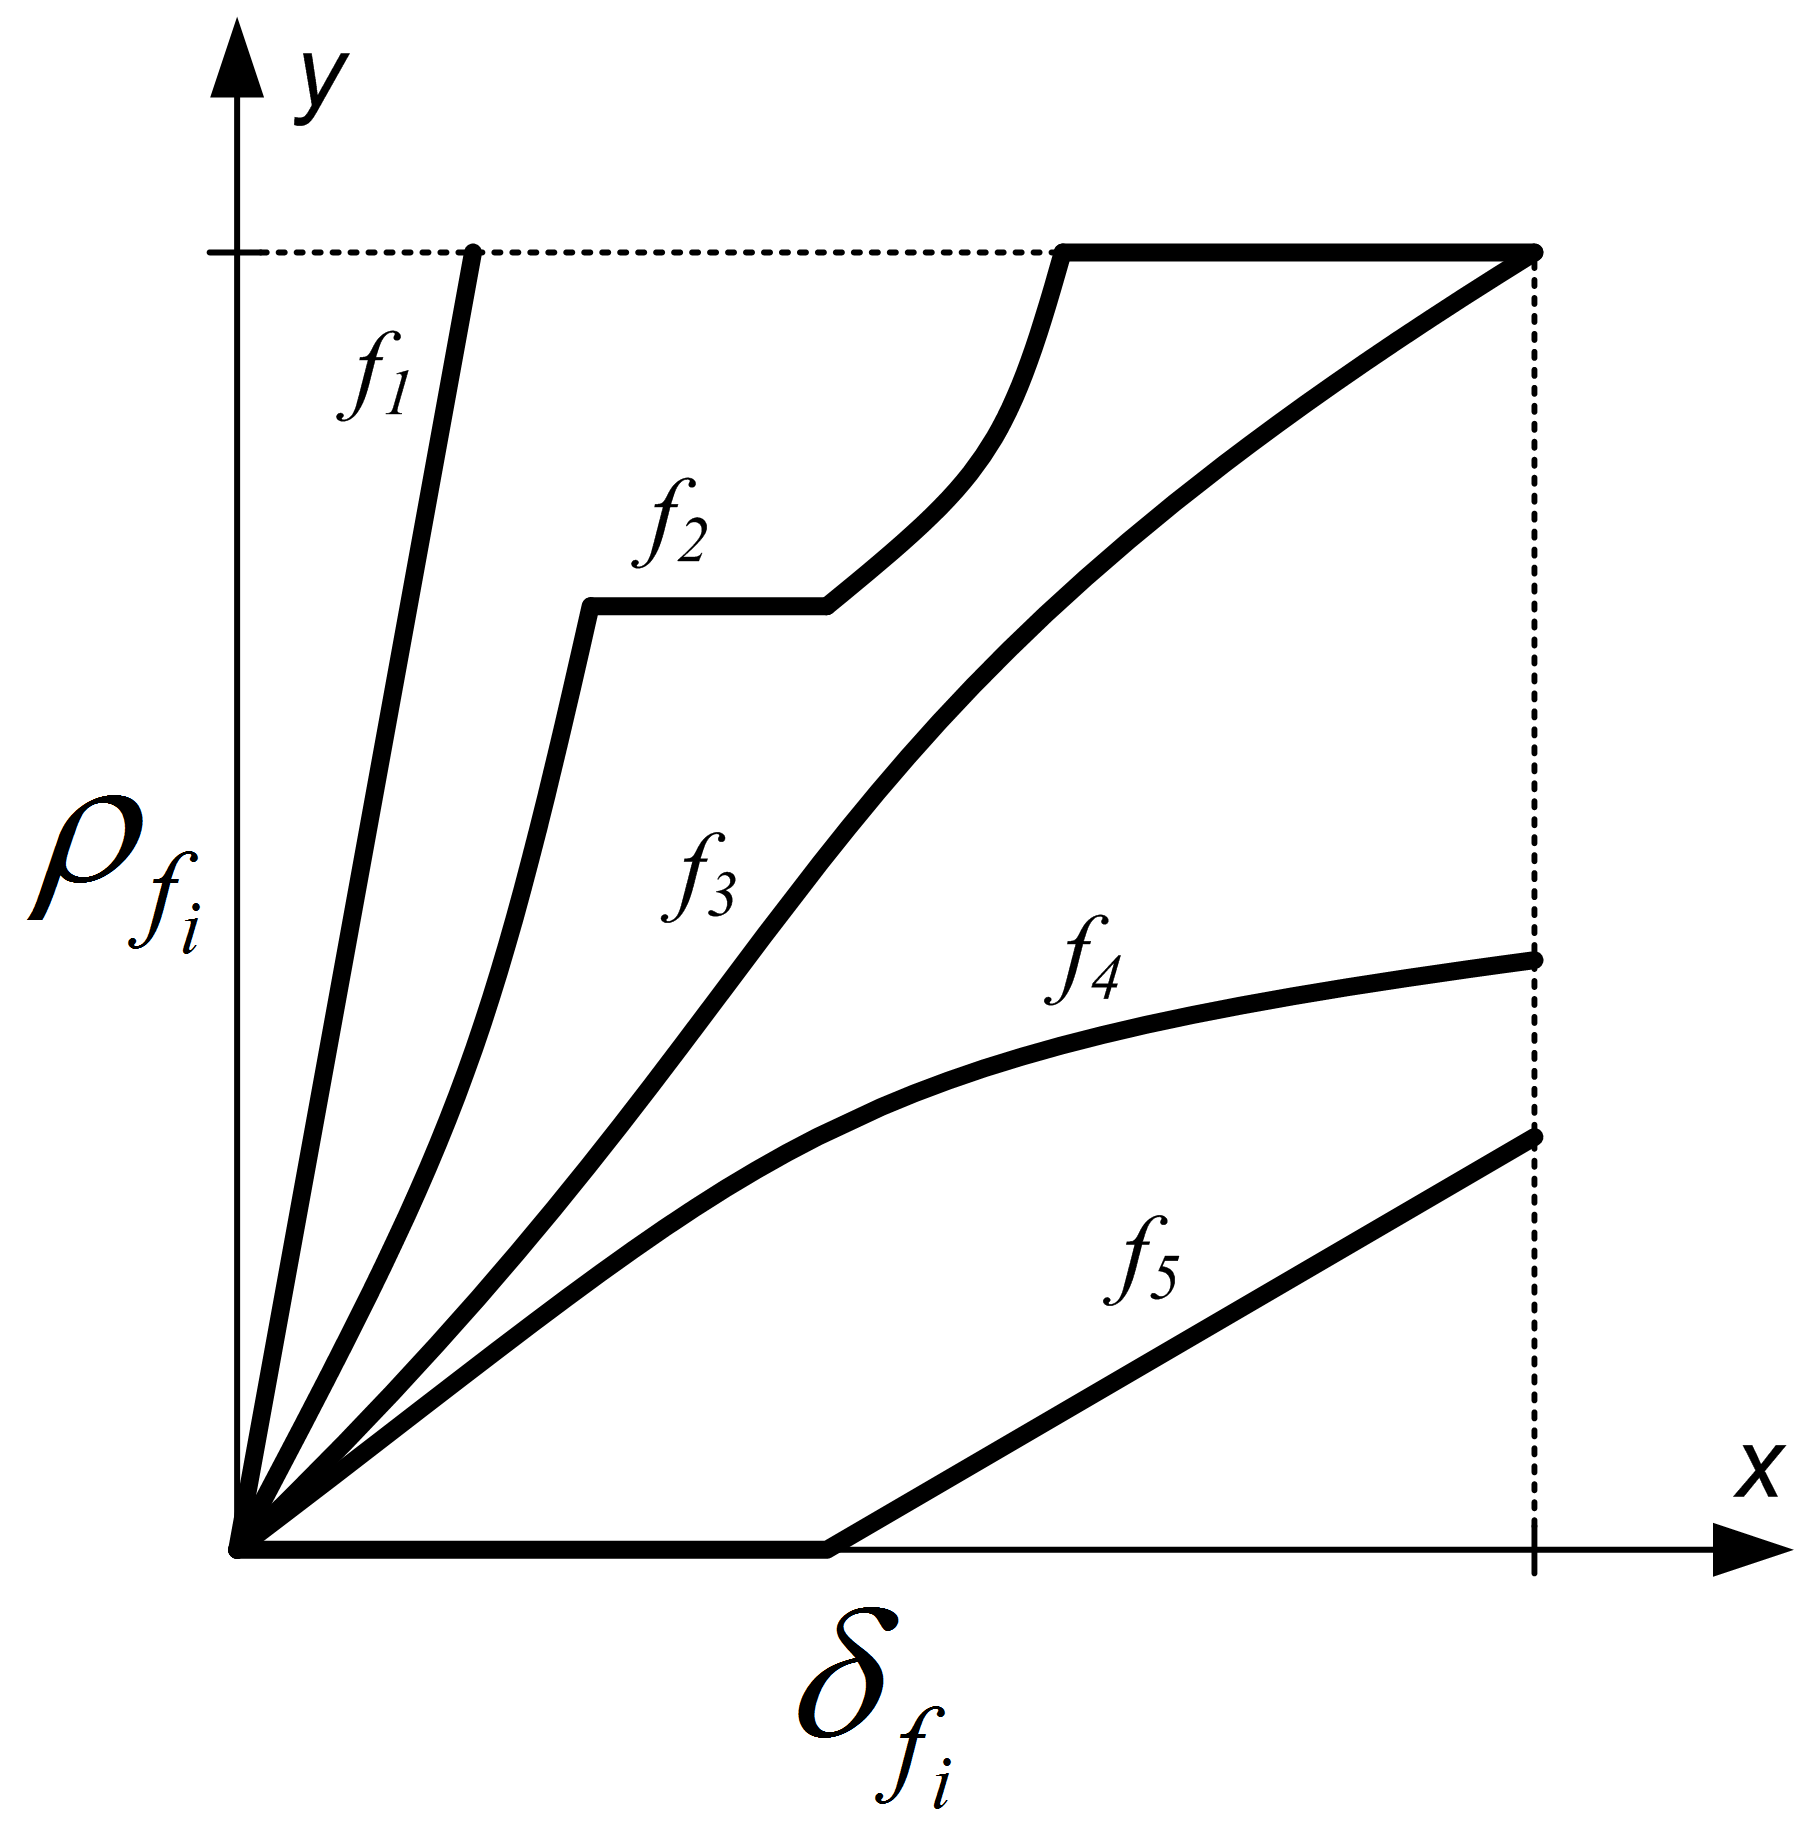
\includegraphics{fig/functionProps}
    \caption{Функции}\label{fig:functionProps}
\end{figure} 

\begin{itemize}
    \item Функция $f:\mathbb{N}\to B$ называется \emph{последовательностью}.

    \item Функция $f:A^n\to B$ называется \emph{$n$-местной функцией} из $A$ в $B$. 

    \item Функция $f:A^n\to A$ называется \emph{$n$-местной алгебраической операцией} на множестве $A$. При $n=1$ операция называется \emph{унарной}, при $n=2$ --- \emph{бинарной}, в остальных случаях --- $n$-арной. При $n=0$ операция $f:A^0\to A$ есть множество $\{(\emptyset,a)\}$ для некоторого $a\in A$. В этом случае операцию обычно называют \emph{константой} и отождествляют с $a$.
\end{itemize}


\section*{Задания}
\addcontentsline{toc}{section}{Задания}

\begin{enumerate}
    \item Задайте матрицу смежности бинарного отношения $\subseteq$ на элементах множества $2^M$, где $M=\{a,b,c\}$.

    \item Задать бинарное отношение $P$ орграфом, матрицей смежности и перечислением пар.
    \begin{enumerate}
        \item  $P\subset A\times B$, $A=\{1,3,5,7\}$, $B=\{2,4,6\}$, $P=\{(a,b)|a+b=9\}$.
        \item  $P\subset A\times B$, $A=\{1,3,5,7\}$, $B=\{2,4,6\}$, $P=\{(a,b)|a<b\}$.
    
        \item $P\subset A^2$, $A=\{1,2,3,4\}$, $P=\{(a,b)|a+2b\equiv 1\pmod{2}\}$.
        \item $P\subset \mathbb{N}^2$, $P=\{(a,b)|2a+b=9,a\neq 0\}$.
        \item $P\subset \mathbb{N}^2$, $P=\{(a,b)|a+b<5\}$.
        
        \item $P\subset \mathbb{N}^2$, $P=\{(x,y)|(x^2=y)\land (0\leq y\leq 100)\}$.
        \item $P\subset \mathbb{N}^2$, $P=\{(x,y)|(x\cdot z^2=y)\land (z\in\mathbb{N})\land (0\leq y\leq 100)\}$.        
    \end{enumerate}
    
    
    \item Задать отношение <<возможен ход с клетки $c_1$ на клетку $c_2$>> (определив множество пар координат с помощью характеристического предиката) клеток шахматной доски (их координат) $c_1=(x_1,y_1)$ и $c_2=(x_2,y_2)$ для следующей шахматной фигуры:
    \begin{enumerate}
        \item пешка;
        \item офицер;
        \item ладья;
        \item конь;
        \item король;
        \item ферзь.
    \end{enumerate}
    
    \item Даны два отношения $P=\{(0,1),(1,2),(2,3),(0,4),(1,5),(2,0)\}$ и $Q=\{(0,0),(1,1),(2,0),(3,1),(4,0),(5,1)\}$. Представить каждое матрицей смежности, найти отношение $PQ$ и построить соответствующий ему орграф.
    
    
    \item Бинарное отношение $P$ на множестве $A=\{1,2,3,4\}$ задано графом.
    \[
        \begin{array}{c}
            {
                \xymatrix{
                    1
                        &2 \ar@{->}[l]
                            \\
                    4 \ar@{->}[r]
                        &3 \ar@{->}[u]
                }    
            }\\
            P
        \end{array}
    \]
    
    Необходимо задать его аналитическим описанием, перечислением пар и матрицей смежности.
    
    
    \item Два бинарных отношения $P$ и $Q$ на множестве $\{0,1,2,3\}$ заданы графами. Определить, проведя вычисления на матрицах смежности, графы отношений $PQ$ и $QP$.
    \[
        \begin{array}{cc}
            \begin{array}{c}
                {
                    \xymatrix{
                        0  \ar@{->}[r]
                            &1 \ar@{->}[d]
                                \\
                        3 \ar@{->}[u]
                            &2 \ar@{->}[l]
                    }    
                }\\
                P
            \end{array}
            &
            \begin{array}{c}
                {
                    \xymatrix{
                        0  \ar@{->}[dr]
                            &1 \ar@{->}[l]
                                \\
                        3 \ar@{->}[ur]
                            &2 \ar@{->}[l]
                    }    
                }\\
                Q
            \end{array}
        \end{array}
    \]

    \item В модулярной арифметике все вычисления происходят <<по фиксированному модулю>> $p$. Т.е. все натуральные аргументы операций изменяются в пределах от $0$ до $p-1$ а результат получается как остаток от деления на $p$. Например: $4+3\equiv 2\pmod{5}$. Далее приведен граф $P$ унарной операции \emph{инкремент} по модулю 5.
    \[
        \begin{array}{c}
            {\xymatrix{
                *{}  
                    &*{} 
                        &1  \ar@{->}[drr]
                            &*{} 
                                &*{}  
                                    \\
                0  \ar@{->}[urr]
                    &*{}  
                        &*{}  
                            &*{}  
                                &2  \ar@{->}[dl]
                                    \\
                *{}  
                    &4  \ar@{->}[ul]
                        &*{}  
                            &3  \ar@{->}[ll]
                                &*{}  
            }}\\
            P
        \end{array}
    \]
    Найти $P^2,P^3,P^4,P^5$ и объяснить словесно, какой унарной операции эти степени инкремента соответствуют.
    
    \item Доказать, что для бинарных отношений $P,Q$ справедливо:
    \begin{enumerate}
        \item $(P^{-1})^{-1}=P$;
        \item $(P\cdot Q)^{-1}=Q^{-1}\cdot P^{-1}$;
        \item $(P\cdot Q)\cdot R=P\cdot(Q\cdot R)$;
        \item $P\cdot Q\neq Q\cdot P$.
    \end{enumerate}
    
    \item Пусть $f(x)=x^2+2x+2$ и $g(x)=\sin(x)$. Найти:
    \begin{enumerate}
        \item $(f\cdot g)(x)$;
        \item $(g\cdot f)(x)$;
        \item $(g\cdot f^{-1})(x)$;
        \item $(f^{-1}\cdot g)(x)$;
    \end{enumerate}
    
    \item Какими свойствами (инъективности, сюръективности, биективности) обладает функция $f:\mathbb{R}\to\mathbb{R}$:
    \begin{enumerate}
        \item $f(x)=e^x$;
        \item $f(x)=x\cdot \sin{(x)}$;
        \item $f(x)=2x-1$;
        \item $f(x)=x^2-1$;
        \item $f(x)=x^3-1$;
        \item $f(x)=2x^3-3x^2+1$.
    \end{enumerate}
    
    Привести примеры частичных функций $f$.
    
    \item Доказать, что:
    \begin{enumerate}
        \item если $f:A\to B$ и $g:B\to C$, то $f\cdot g:A\to C$;
        
        \item если $f:A\xrightarrow{\text{на}} B$ и $g:B\xrightarrow{\text{на}} C$, то $f\cdot g:A\xrightarrow{\text{на}} C$;
        
        \item если $f:A\xrightarrow{\text{в}} B$ и $g:B\xrightarrow{\text{в}} C$, то $f\cdot g:A\xrightarrow{\text{в}} C$;
        
        \item если $f:A\leftrightarrow B$ и $g:B\leftrightarrow C$, то $f\cdot g:A\leftrightarrow C$;
        
        \item если $f:A\leftrightarrow B$, то $f^{-1}:B\leftrightarrow A$, то $f\cdot f^{-1}=I_A$ и $f^{-1}\cdot f=I_B$.
    \end{enumerate}

    \item Очень важным элементом в системах пакетной передачи данных является коммутатор --- устройство, позволяющее передавать пакеты информации в нужные каналы. При этом пакет информации содержит <<адрес>> канала назначения в служебных полях. Каждый элемент $i$-го слоя коммутационной сети (см. рис. \ref{fig:rel:commutate}) автономен и работает так: получив пакет (пакеты поступают на входы $a,b$), элемент просматривает $i$-й бит адреса $a_i$ канала назначения и направляет пакет на выход $c$, если $a_i=0$, или на выход $d$, если $a_i=1$. 
    
    На рисунке \ref{fig:rel:commutate} приведена коммутационная сеть на восемь входов и восемь выходов, состоящая из трех четырехэлементных слоёв. Задав для каждого слоя отношение <<вход $x$ может поступать на выход $y$>> и функции перестановки для соседних слоев <<i-й выход слоя поступает на j-й вход следующиго слоя>>, формально докажите, что пакет, поступивший на любой вход первого слоя может выйти на любой выход третьего.

    \begin{figure}
        \centering
        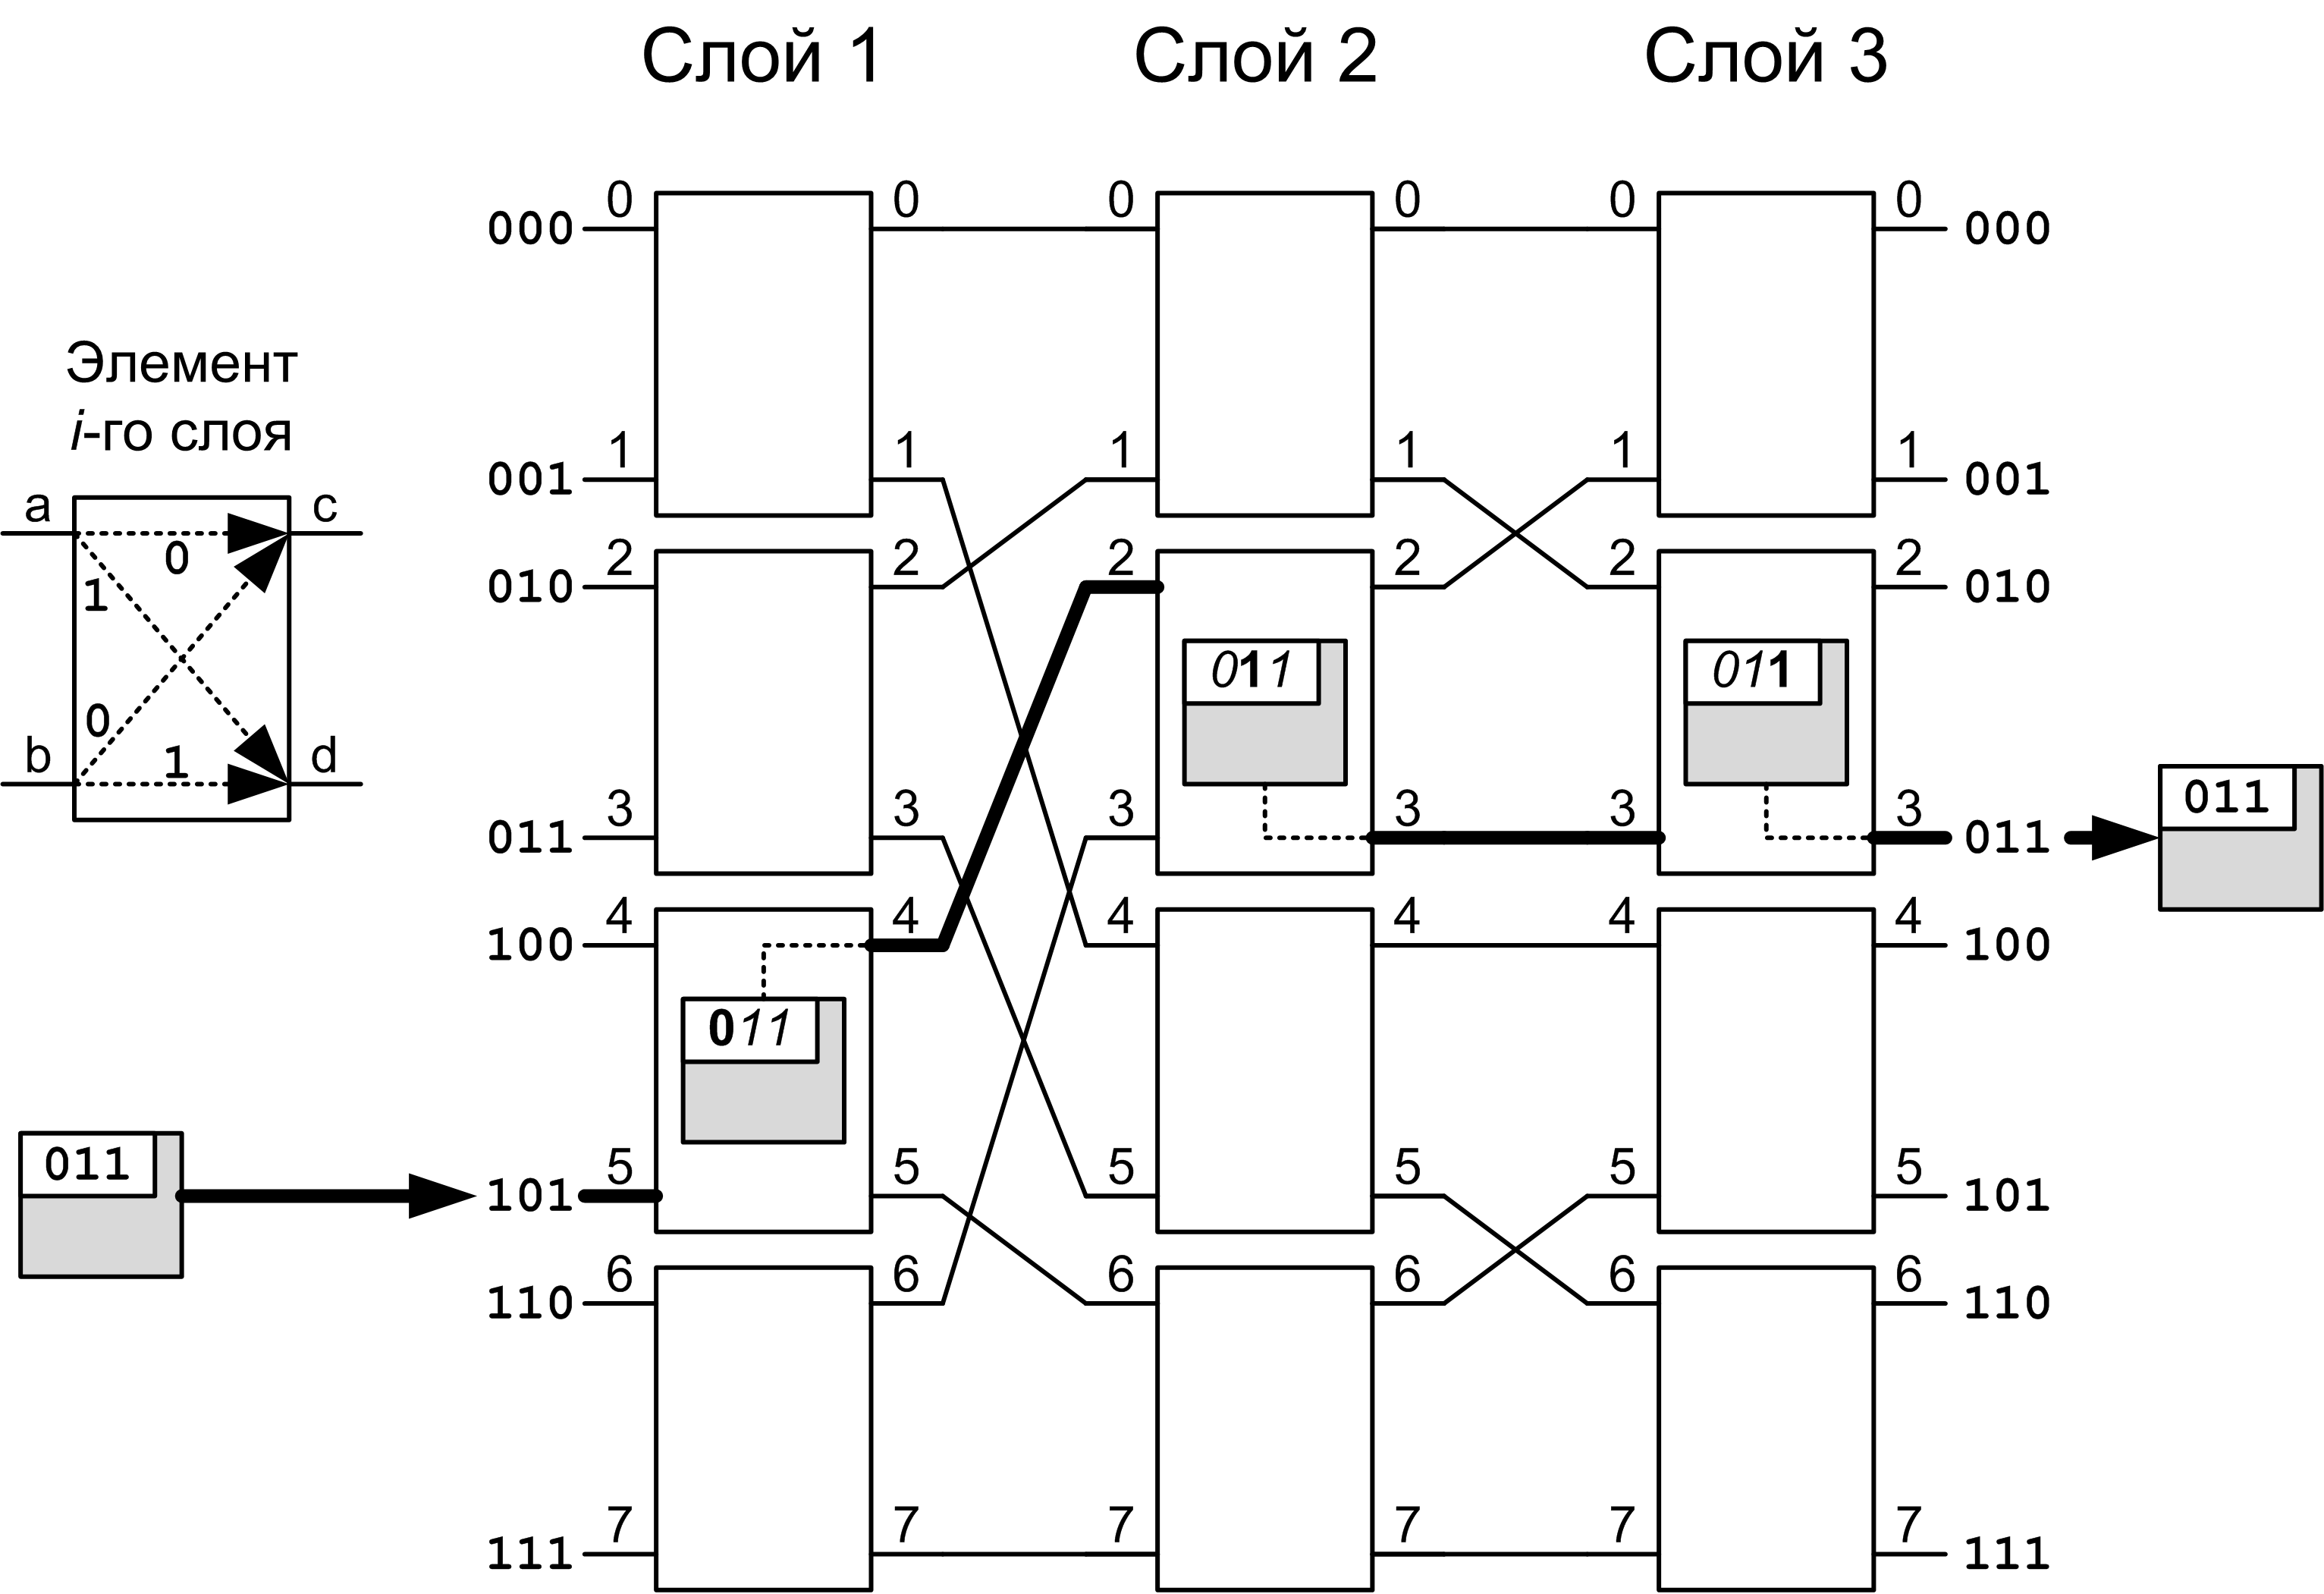
\includegraphics[width=0.7\textwidth]{fig/commutate}
        \caption{Сеть коммутации $8\times 8$}
        \label{fig:rel:commutate}
    \end{figure} 
    
\end{enumerate}
